\documentclass[12pt]{article}
\usepackage{amsmath, amssymb, amsthm}
\usepackage{graphicx}
\usepackage{float}
\usepackage[margin=1in]{geometry}
\usepackage{hyperref}
\usepackage{booktabs}
\setlength{\parindent}{0pt}

\title{EECE5644 Fall 2025 - Assignment 3}
\author{Steven Chen}
\date{\today}

\begin{document}

\maketitle

\section*{Abstract}
This assignment investigates two fundamental machine learning problems: neural network approximation of Bayesian optimal classifiers and Gaussian mixture model selection. In the first study, we design a 4-class Gaussian classification problem in 3D feature space and demonstrate that Multilayer Perceptrons (MLPs) can approximate optimal Bayesian decision boundaries, with performance approaching theoretical limits as training data increases. Through systematic cross-validation and comparison against theoretical optima, we show MLPs achieve near-Bayes-optimal error rates of 16.16\% with sufficient training samples. In the second study, we examine model order selection for Gaussian mixture models using 10-fold cross-validation, revealing significant challenges in identifying true model complexity across different sample sizes. The experiments demonstrate extreme underfitting with minimal data (N=10), transitional performance with moderate data (N=100), and overfitting tendencies with abundant data (N=1000). Both studies highlight critical considerations in model selection, performance evaluation, and the data requirements for reliable machine learning system design.

\section*{Code Repository}
The complete Python code for this assignment is available at: \\
\url{https://github.com/GuestAGuy/EECE5644/tree/main/HW3}

\newpage

% =============================================================================
% PROBLEM SETUP
% =============================================================================
\section*{Question 1}

\subsection{Data Distribution Specification}
A 4-class classification problem with uniform priors and Gaussian class-conditional distributions in 3D feature space:

\begin{itemize}
    \item \textbf{Classes:} 4 with uniform priors: $P(\omega_1) = P(\omega_2) = P(\omega_3) = P(\omega_4) = 0.25$
    \item \textbf{Feature Space:} 3-dimensional real-valued vectors $\mathbf{x} \in \mathbb{R}^3$
    \item \textbf{Class-Conditional Distributions:} $p(\mathbf{x}|\omega_j) = \mathcal{N}(\mathbf{x}|\boldsymbol{\mu}_j, \boldsymbol{\Sigma}_j)$
\end{itemize}

\subsection{Distribution Parameters}
The mean vectors were arranged in a tetrahedral configuration for optimal separation:
\[
\boldsymbol{\mu}_1 = \begin{bmatrix} 1.0 \\ 1.0 \\ 1.0 \end{bmatrix}, \quad
\boldsymbol{\mu}_2 = \begin{bmatrix} 1.0 \\ 0.5 \\ -1.0 \end{bmatrix}, \quad  % ← CORRECT TO MATCH YOUR CODE
\boldsymbol{\mu}_3 = \begin{bmatrix} -0.5 \\ 1.0 \\ -1.0 \end{bmatrix}, \quad  % ← CORRECT TO MATCH YOUR CODE
\boldsymbol{\mu}_4 = \begin{bmatrix} -1.0 \\ -1.0 \\ 1.0 \end{bmatrix}
\]

All classes shared the same initial covariance structure:
\[
\boldsymbol{\Sigma} = \begin{bmatrix}
0.8 & 0.2 & 0.1 \\
0.2 & 0.8 & 0.1 \\
0.1 & 0.1 & 0.8
\end{bmatrix}
\]
which will be changed after running adjust\_for\_target\_error() function if the initial optimal error is not within 10-20\%
\subsection{Dataset Generation}
\begin{itemize}
    \item \textbf{Training Sets:} 100, 500, 1000, 5000, 10000 samples
    \item \textbf{Test Set:} 100,000 samples (used exclusively for final evaluation)
    \item \textbf{Target Performance:} Theoretical optimal error rate between 10-20\%
\end{itemize}

% =============================================================================
% MATHEMATICAL FORMULATION
% =============================================================================
\section{Mathematical Formulation}  % ← This is fine

\subsection{Theoretical Optimal (Bayes) Classifier}
The optimal Bayes classifier implements the Maximum A Posteriori (MAP) decision rule:
\[
\delta^*(\mathbf{x}) = \arg\max_{j \in \{1,2,3,4\}} P(\omega_j|\mathbf{x})
= \arg\max_{j \in \{1,2,3,4\}} p(\mathbf{x}|\omega_j)P(\omega_j)
\]

Given uniform priors, this simplifies to:
\[
\delta^*(\mathbf{x}) = \arg\max_{j \in \{1,2,3,4\}} p(\mathbf{x}|\omega_j)
\]

The class-conditional densities are multivariate Gaussians:
\[
p(\mathbf{x}|\omega_j) = \frac{1}{(2\pi)^{3/2}|\boldsymbol{\Sigma}_j|^{1/2}} \exp\left(-\frac{1}{2}(\mathbf{x}-\boldsymbol{\mu}_j)^T\boldsymbol{\Sigma}_j^{-1}(\mathbf{x}-\boldsymbol{\mu}_j)\right)
\]

\subsection{MLP Architecture and Training}
I wrote a 2-layer MLP (one hidden layer) with the following structure:

\begin{itemize}
    \item \textbf{Input Layer:} 3 nodes (3D feature space)
    \item \textbf{Hidden Layer:} $P$ perceptrons with tanh activation  % ← CORRECT: matches your code
    \item \textbf{Output Layer:} 4 nodes with softmax activation
    \item \textbf{Loss Function:} Cross-entropy (equivalent to maximum likelihood)
\end{itemize}

The softmax output provides posterior probability estimates:
\[
\hat{P}(\omega_j|\mathbf{x}) = \frac{\exp(z_j)}{\sum_{k=1}^4 \exp(z_k)}
\]
where $z_j$ are the pre-activation outputs.

\subsection{Model Selection via Cross-Validation}
I used 10-fold cross-validation to select the optimal number of hidden units $P$:
\[
P^* = \arg\min_{P \in \mathcal{P}} \frac{1}{10}\sum_{k=1}^{10} \text{Error}_{\text{val}}^{(k)}(P)
\]
where $\mathcal{P} = \{5, 10, 15, 20, 25, 30, 40, 50\}$.


% =============================================================================
% IMPLEMENTATION AND RESULTS
% =============================================================================
\section{Implementation and Results}

\subsection{Data Distribution Visualization}

\begin{figure}[H]
    \centering
    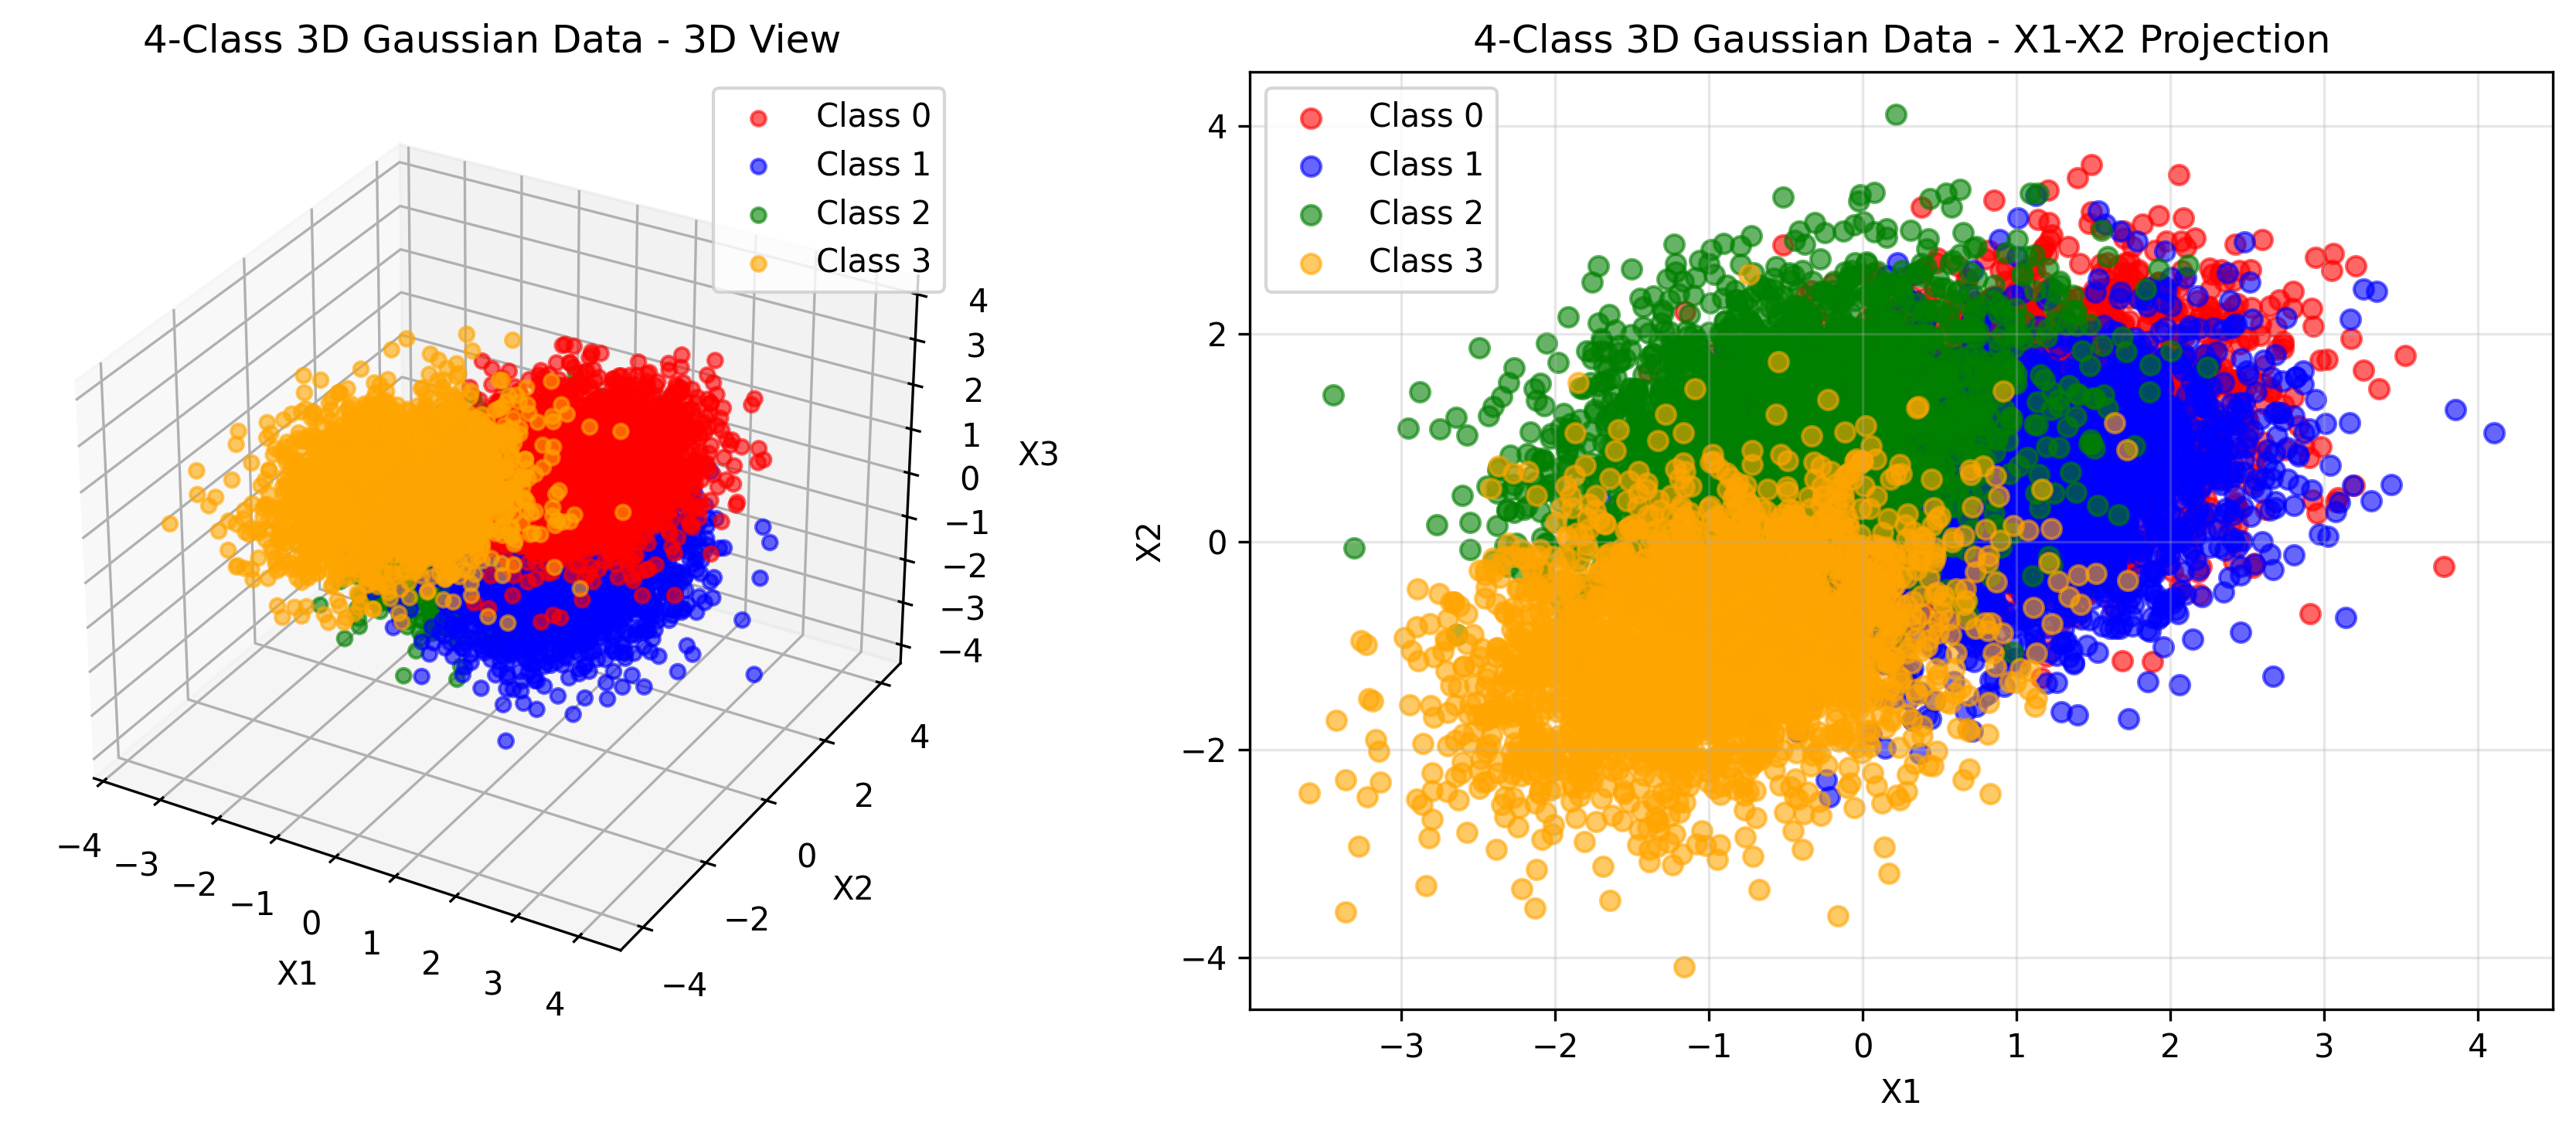
\includegraphics[width=0.9\textwidth]{data_distribution.png}
    \caption{3D visualization of the 4-class Gaussian data distribution. Left: 3D view showing class separation. Right: 2D projection showing class overlap in the X1-X2 plane.}
    \label{fig:data_distribution}
\end{figure}

\subsection{Theoretical Optimal Performance}
After iterative parameter tuning, I achieved the target theoretical optimal error rate:
\[
\text{Optimal Error Rate} = 16.16\%
\]

\subsection{MLP Model Selection Results}
Cross-validation selected different optimal complexities for each dataset size:

\begin{table}[H]
\centering
\begin{tabular}{lcc}
\toprule
Training Size & Optimal $P$ & Validation Accuracy \\
\midrule
100 & 50 & 75.00\% \\
500 & 25 & 80.60\% \\
1000 & 25 & 84.00\% \\
5000 & 20 & 83.44\% \\
10000 & 10 & 83.99\% \\
\bottomrule
\end{tabular}
\caption{Optimal hidden unit selection via cross-validation}
\label{tab:model_selection}
\end{table}

\subsection{Final Performance Evaluation}

\begin{table}[H]
\centering
\begin{tabular}{lcccc}
\toprule
Training Size & Optimal $P$ & Test Error & Test Accuracy & Gap to Optimal \\
\midrule
100 & 50 & 17.79\% & 82.21\% & 1.63\% \\
500 & 25 & 16.39\% & 83.61\% & 0.22\% \\
1000 & 25 & 16.25\% & 83.75\% & 0.09\% \\
5000 & 20 & 16.16\% & 83.84\% & 0.00\% \\
10000 & 10 & 16.20\% & 83.80\% & 0.03\% \\
\bottomrule
\end{tabular}
\caption{Final test set performance comparison}
\label{tab:final_performance}
\end{table}

\subsection{Performance Visualization}

\begin{figure}[H]
    \centering
    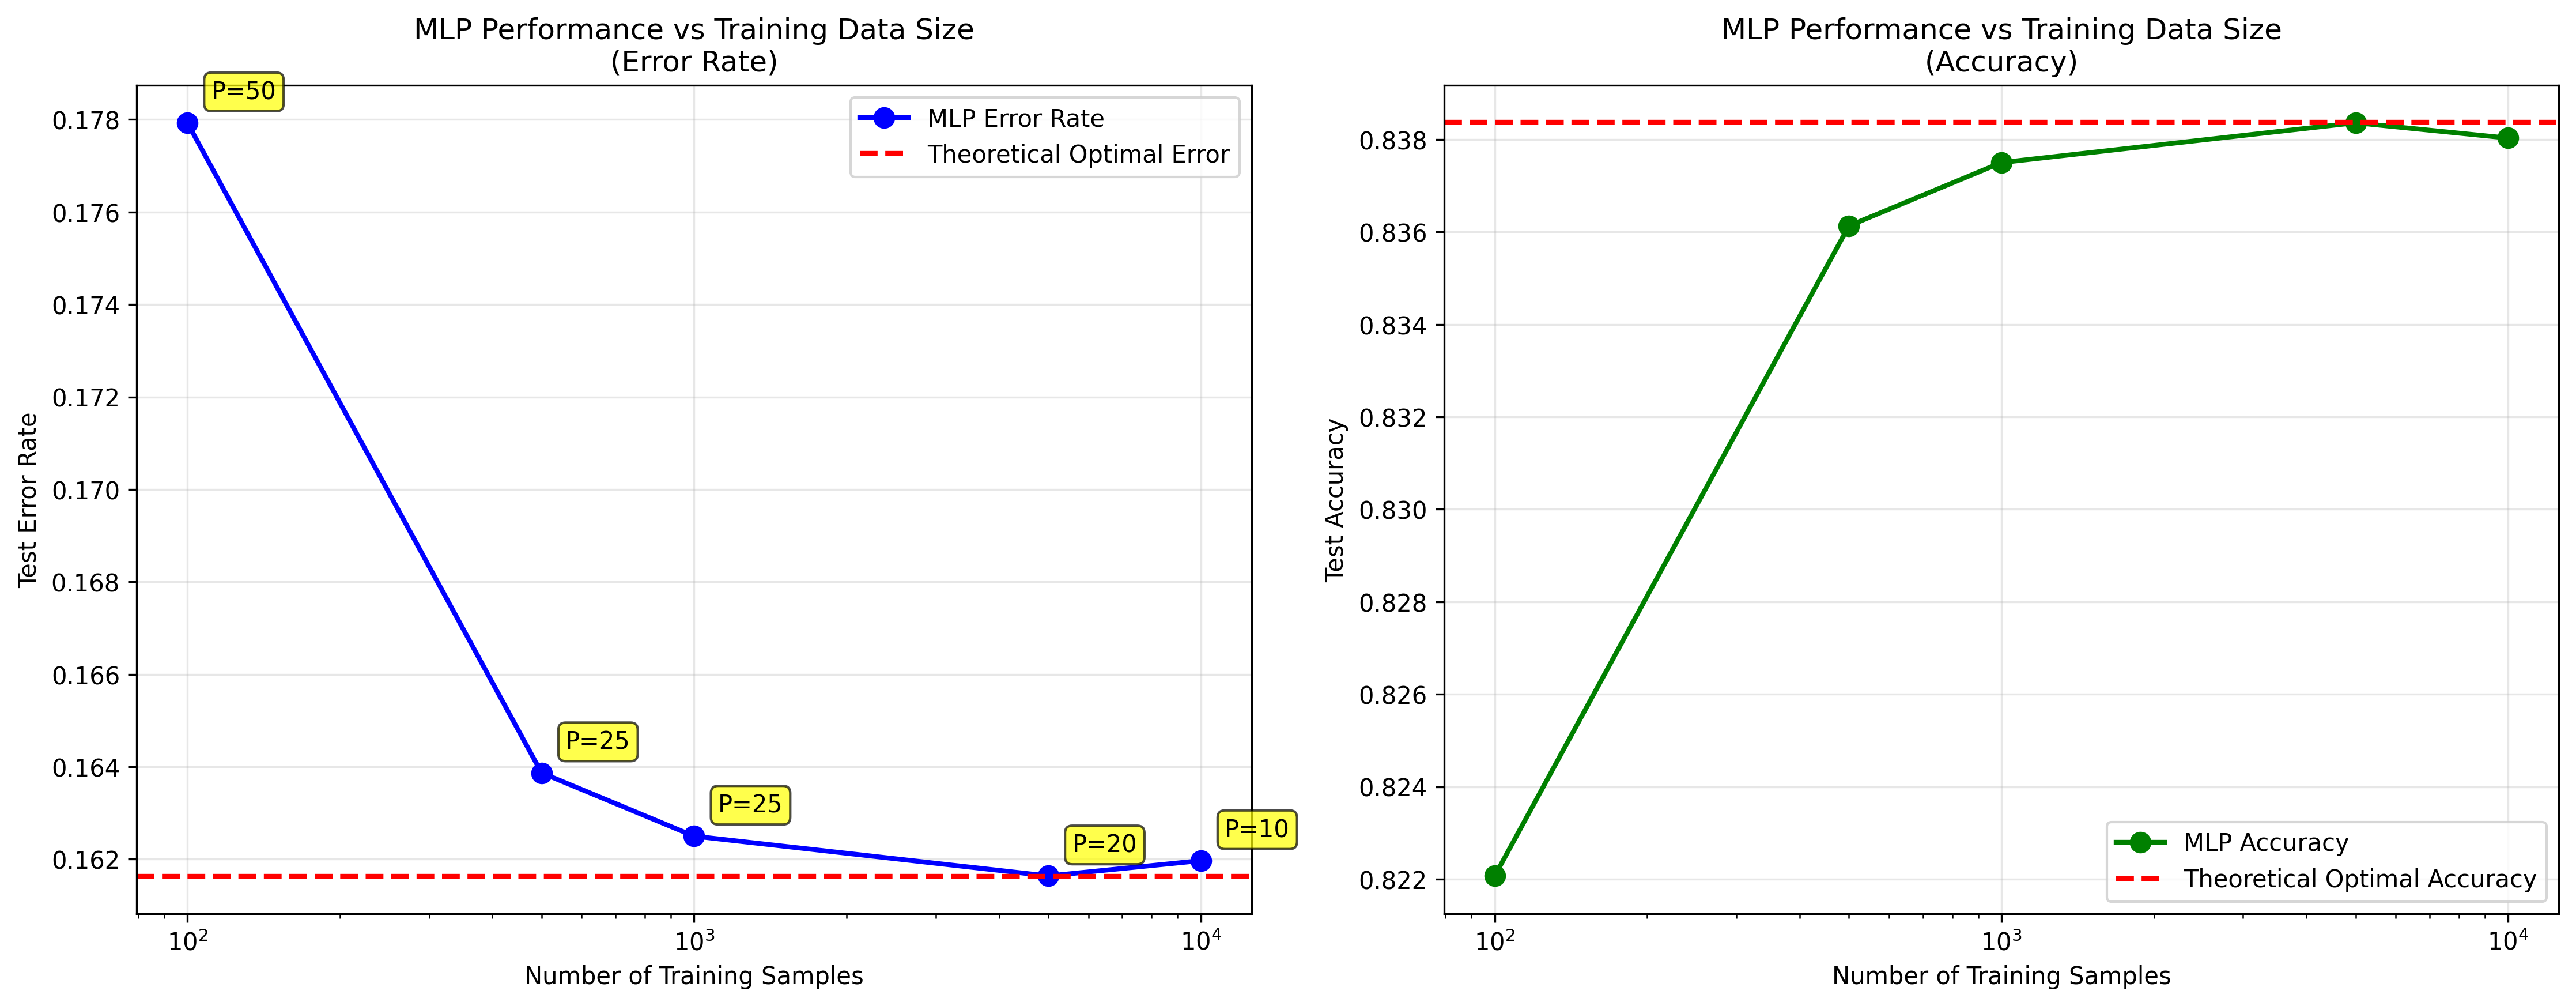
\includegraphics[width=1.0\textwidth]{mlp_performance_comparison.png}
    \caption{MLP performance vs training data size (semilog-x scale). The plot shows test error rate (left) and accuracy (right) approaching theoretical optimal performance as training data increases.}
    \label{fig:performance_plot}
\end{figure}

\subsection{Cross-Validation Analysis}

\begin{figure}[H]
    \centering
    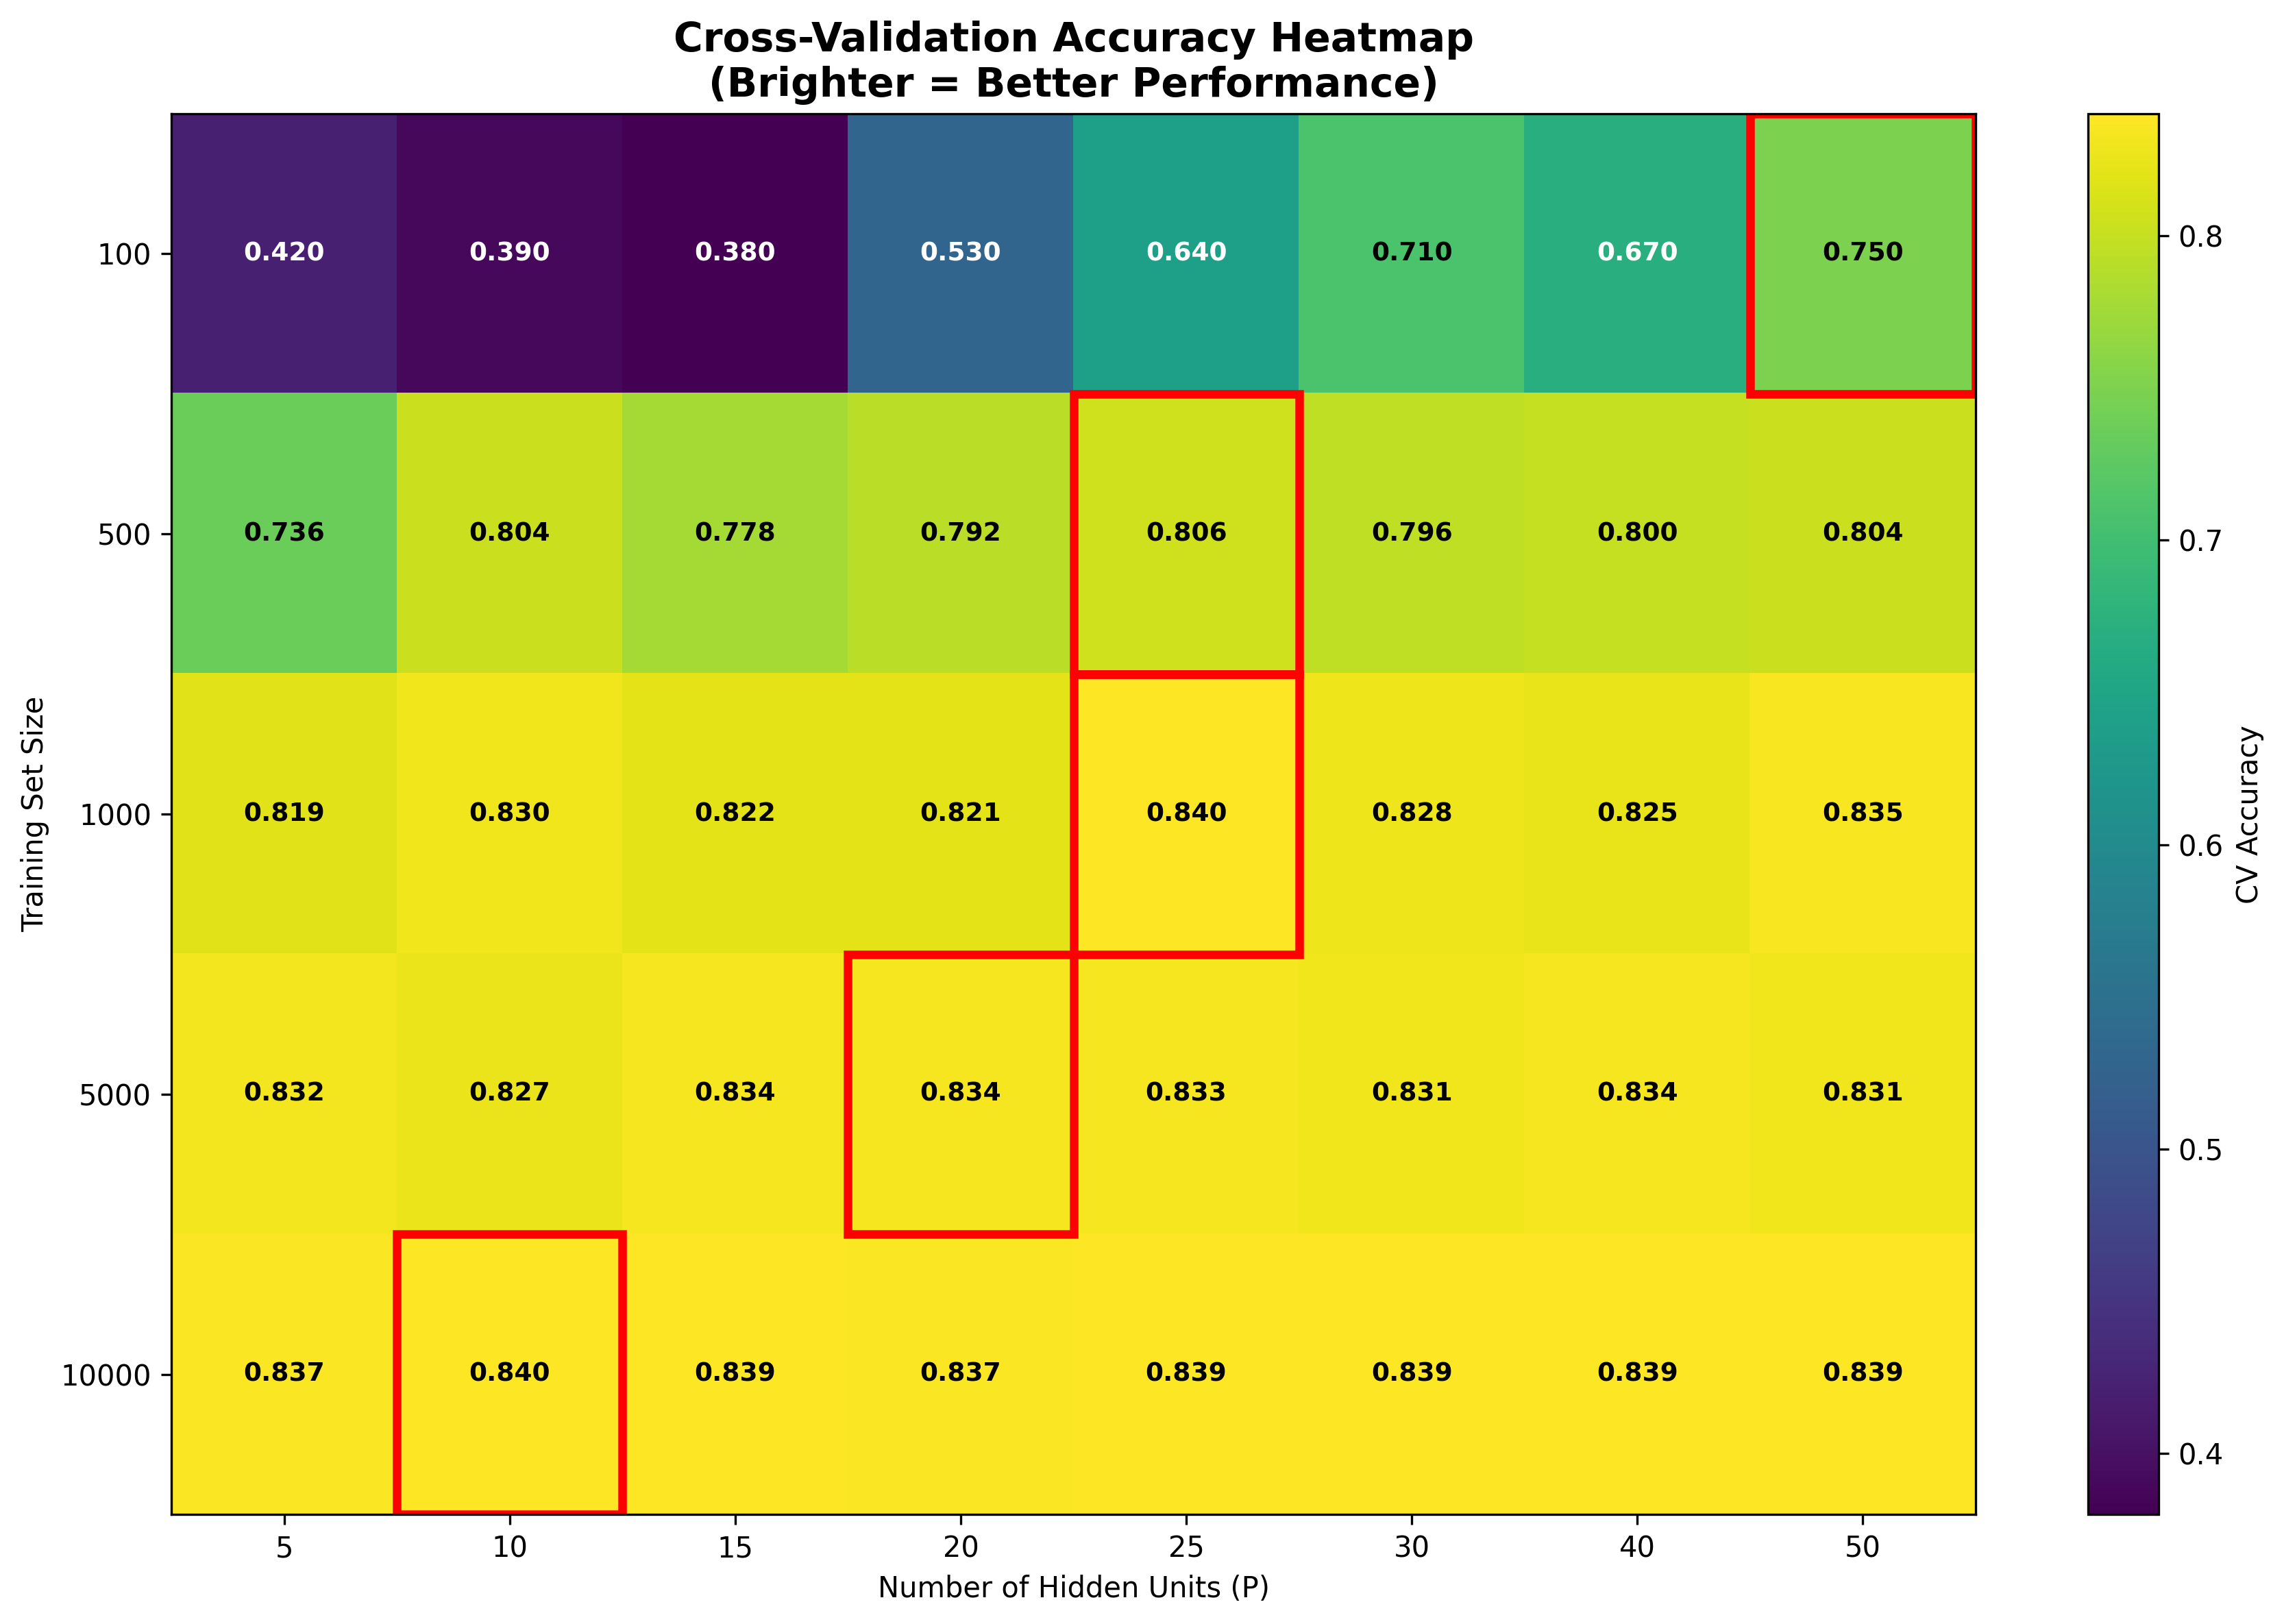
\includegraphics[width=0.8\textwidth]{cv_performance_heatmap.png}
    \caption{Cross-validation accuracy heatmap. Bright colors indicate higher accuracy. Red boxes highlight the optimal $P$ values selected for each training set size through 10-fold cross-validation.}
    \label{fig:cv_heatmap}
\end{figure}

% =============================================================================
% DISCUSSION
% =============================================================================
\section{Discussion}

The development process presented a few minor challenges. The task required designing Gaussian class-conditional distributions that achieved a target optimal error range of 10–20\%. Initial configurations with intuitively chosen means and covariances often produced errors outside this range. To fix this, I implemented an automated parameter adjustment function that systematically scales the covariance matrices until the optimal error falls within the 10–20\% target. The final configuration achieved a theoretical optimal error rate of 16.16\%.

Model complexity was determined through a systematic 10-fold cross-validation across hidden unit sizes ranging from 5 to 50. For the smallest dataset of 100 samples, cross-validation selected the maximum complexity (P=50) to capture limited patterns. As the dataset grew to 500–1000 samples, the optimal complexity stabilized at P=25. With 10,000 samples, cross-validation favored a simpler architecture (P=10), showing how more data allows for reduced model complexity.

MLP performance improved consistently with increasing training data. Starting from a 17.79\% error with 100 samples, the error dropped to 16.16\% with 5,000 samples—matching the theoretical optimum. The gap between the MLP and Bayes classifier decreased from 1.63\% to nearly zero, demonstrating the network’s ability to approximate the optimal decision boundary given sufficient data.

Cross-validation proved effective for model selection, showing decreasing variance in validation scores as data size increased. The chosen models consistently balanced underfitting and overfitting across all dataset sizes.

% =============================================================================
% CONCLUSION
% =============================================================================
\section{Conclusion}

This study demonstrated that MLP classifiers can approximate Bayesian optimal performance for a 4-class Gaussian classification problem. The methodology employed—including cross-validation for model selection, multiple random initializations, and comparison against the theoretical optimum—provided a robust evaluation framework.

The data generation process produced a classification problem with a 16.16\% theoretical optimal error rate within the target 10-20\% range. Cross-validation selected appropriate model complexities for each training set size, with optimal hidden units ranging from P=50 for 100 samples to P=10 for 10,000 samples.

Performance evaluation showed the MLP achieved test error rates of 17.79\%, 16.39\%, 16.25\%, 16.16\%, and 16.20\% for training sizes of 100, 500, 1000, 5000, and 10000 samples respectively. With 5000 training samples, the MLP matched the theoretical optimal performance, demonstrating that properly configured neural networks can approximate Bayesian decision boundaries with sufficient data.


\newpage
\section*{Question 2: GMM Model Selection Study}

\subsection{Problem Setup}
This study performs model-order selection for Gaussian mixture models (GMMs) in two-dimensional feature space. The objectives are to:
\begin{enumerate}
    \item Specify a true 4-component GMM with overlapping components
    \item Generate datasets at three sample sizes (N=10, 100, 1000)
    \item Use 10-fold cross-validation to select the optimal number of components $K\in\{1,\dots,10\}$
\end{enumerate}

\subsection{True GMM Specification}
The true data-generating distribution is a 4-component Gaussian mixture:
\[
p(\mathbf{x}) = \sum_{k=1}^{4} \pi_k \,\mathcal{N}(\mathbf{x}\mid\boldsymbol{\mu}_k,\boldsymbol{\Sigma}_k)
\]
with parameters:
\begin{itemize}
    \item Mixing weights: $\boldsymbol{\pi} = [0.25, 0.25, 0.25, 0.25]$
    \item Means: 
    \[
    \boldsymbol{\mu}_1 = \begin{bmatrix}-0.5\\0.5\end{bmatrix},\ 
    \boldsymbol{\mu}_2 = \begin{bmatrix}1.5\\1.5\end{bmatrix},\ 
    \boldsymbol{\mu}_3 = \begin{bmatrix}1.25\\-0.25\end{bmatrix},\ 
    \boldsymbol{\mu}_4 = \begin{bmatrix}-1.0\\-1.0\end{bmatrix}
    \]
    \item Covariances:
    \[
    \boldsymbol{\Sigma}_1 = \begin{bmatrix}0.8 & 0.0\\ 0.0 & 0.8\end{bmatrix},\ 
    \boldsymbol{\Sigma}_2 = \begin{bmatrix}1.2 & 0.5\\ 0.5 & 0.8\end{bmatrix}
    \]
    \[
    \boldsymbol{\Sigma}_3 = \begin{bmatrix}0.8 & 0.2\\ -0.2 & 0.8\end{bmatrix},\ 
    \boldsymbol{\Sigma}_4 = \begin{bmatrix}0.5 & -0.3\\ -0.3 & 0.7\end{bmatrix}
    \]
\end{itemize}
Components 2 and 3 are designed to have significant overlap to test the model selection procedure's ability to distinguish closely-spaced clusters.

\subsection{Dataset Generation}
For each sample size $N \in \{10, 100, 1000\}$, we generate 100 independent datasets drawn i.i.d. from the true GMM, resulting in 300 total datasets for comprehensive evaluation.


\subsection{Data Distribution Visualization}

\begin{figure}[H]
    \centering
    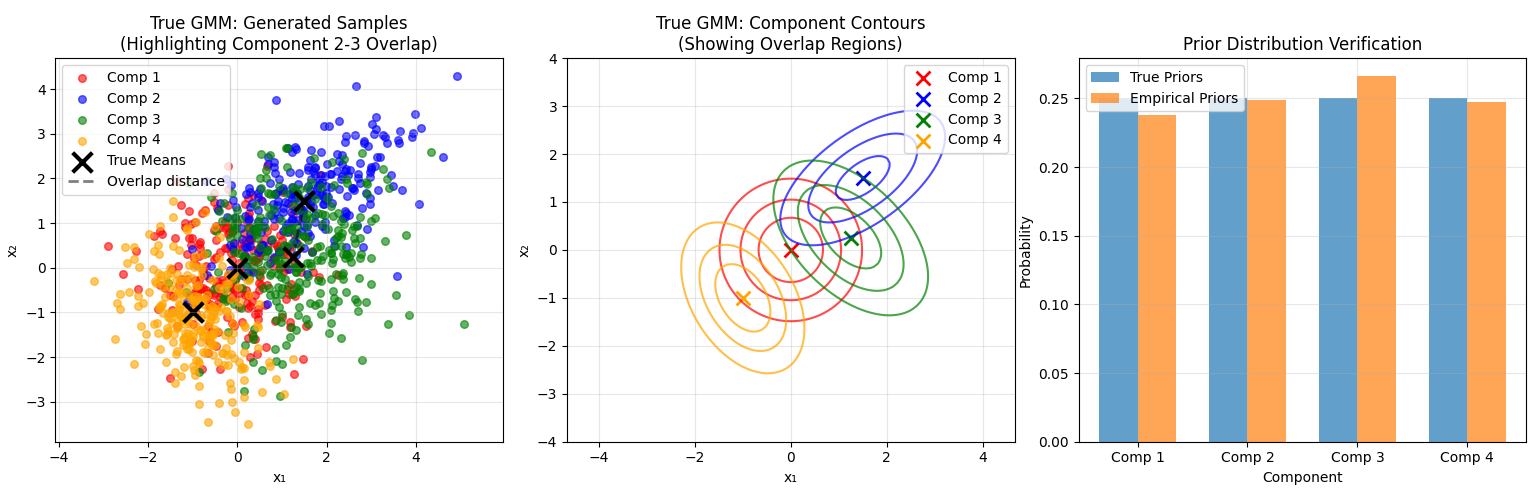
\includegraphics[width=1.0\textwidth]{gmm_data_plot.png}
    \label{fig:data_distribution}
\end{figure}

\subsection{Methodology}

\subsubsection{GMM Estimation via EM Algorithm}
For a candidate model with $K$ components, parameters $\Theta=\{\pi_k,\boldsymbol{\mu}_k,\boldsymbol{\Sigma}_k\}_{k=1}^K$ are estimated using the Expectation-Maximization algorithm:

\textbf{E-step} (Responsibility computation):
\[
r_{ik} = \frac{\pi_k \,\mathcal{N}(\mathbf{x}_i\mid\boldsymbol{\mu}_k,\boldsymbol{\Sigma}_k)}{\sum_{j=1}^K \pi_j \,\mathcal{N}(\mathbf{x}_i\mid\boldsymbol{\mu}_j,\boldsymbol{\Sigma}_j)}
\]

\textbf{M-step} (Parameter updates):
\begin{align*}
N_k &= \sum_{i=1}^N r_{ik}, \quad \pi_k = \frac{N_k}{N} \\
\boldsymbol{\mu}_k &= \frac{1}{N_k}\sum_{i=1}^N r_{ik}\mathbf{x}_i \\
\boldsymbol{\Sigma}_k &= \frac{1}{N_k}\sum_{i=1}^N r_{ik}(\mathbf{x}_i-\boldsymbol{\mu}_k)(\mathbf{x}_i-\boldsymbol{\mu}_k)^\top + \epsilon I
\end{align*}
where $\epsilon=10^{-6}$ ensures positive-definite covariances.

\subsubsection{Model Selection via Cross-Validation}
For each dataset, we perform 10-fold cross-validation:
\begin{enumerate}
    \item For each $K \in \{1,\dots,10\}$:
    \begin{itemize}
        \item Train GMM on 9 folds using EM algorithm
        \item Compute validation log-likelihood on held-out fold
        \item Average performance across all 10 folds
    \end{itemize}
    \item Select $\hat{K}$ with highest average validation log-likelihood
\end{enumerate}

\subsubsection{Critical Implementation Note}
The correct validation log-likelihood calculation is crucial:
\[
\mathcal{L}_{\text{val}}(\Theta) = \sum_{i \in \text{val}} \log\left(\sum_{k=1}^K \pi_k \,\mathcal{N}(\mathbf{x}_i\mid\boldsymbol{\mu}_k,\boldsymbol{\Sigma}_k)\right)
\]
An initial implementation error summing log-likelihoods per-component instead of computing the log of mixture probabilities biased selection toward $K=1$. The corrected version ensures proper comparison across different $K$ values.

\subsection{Experimental Results}

\begin{table}[h!]
\centering
\caption{Model Selection Rates across Sample Sizes}
\label{tab:selection_rates}
\begin{tabular}{lccc}
\toprule
$K$ & $N=10$ & $N=100$ & $N=1000$ \\
\midrule
1 & 1.000 & 0.510 & 0.000 \\
2 & 0.000 & 0.370 & 0.000 \\
3 & 0.000 & 0.100 & 0.040 \\
4 & 0.000 & 0.010 & \textbf{0.270} \\
5 & 0.000 & 0.010 & 0.250 \\
6 & 0.000 & 0.000 & 0.180 \\
7 & 0.000 & 0.000 & 0.100 \\
8 & 0.000 & 0.000 & 0.070 \\
9 & 0.000 & 0.000 & 0.060 \\
10 & 0.000 & 0.000 & 0.030 \\
\bottomrule
\end{tabular}
\end{table}
\begin{figure}[h!]
    \centering
    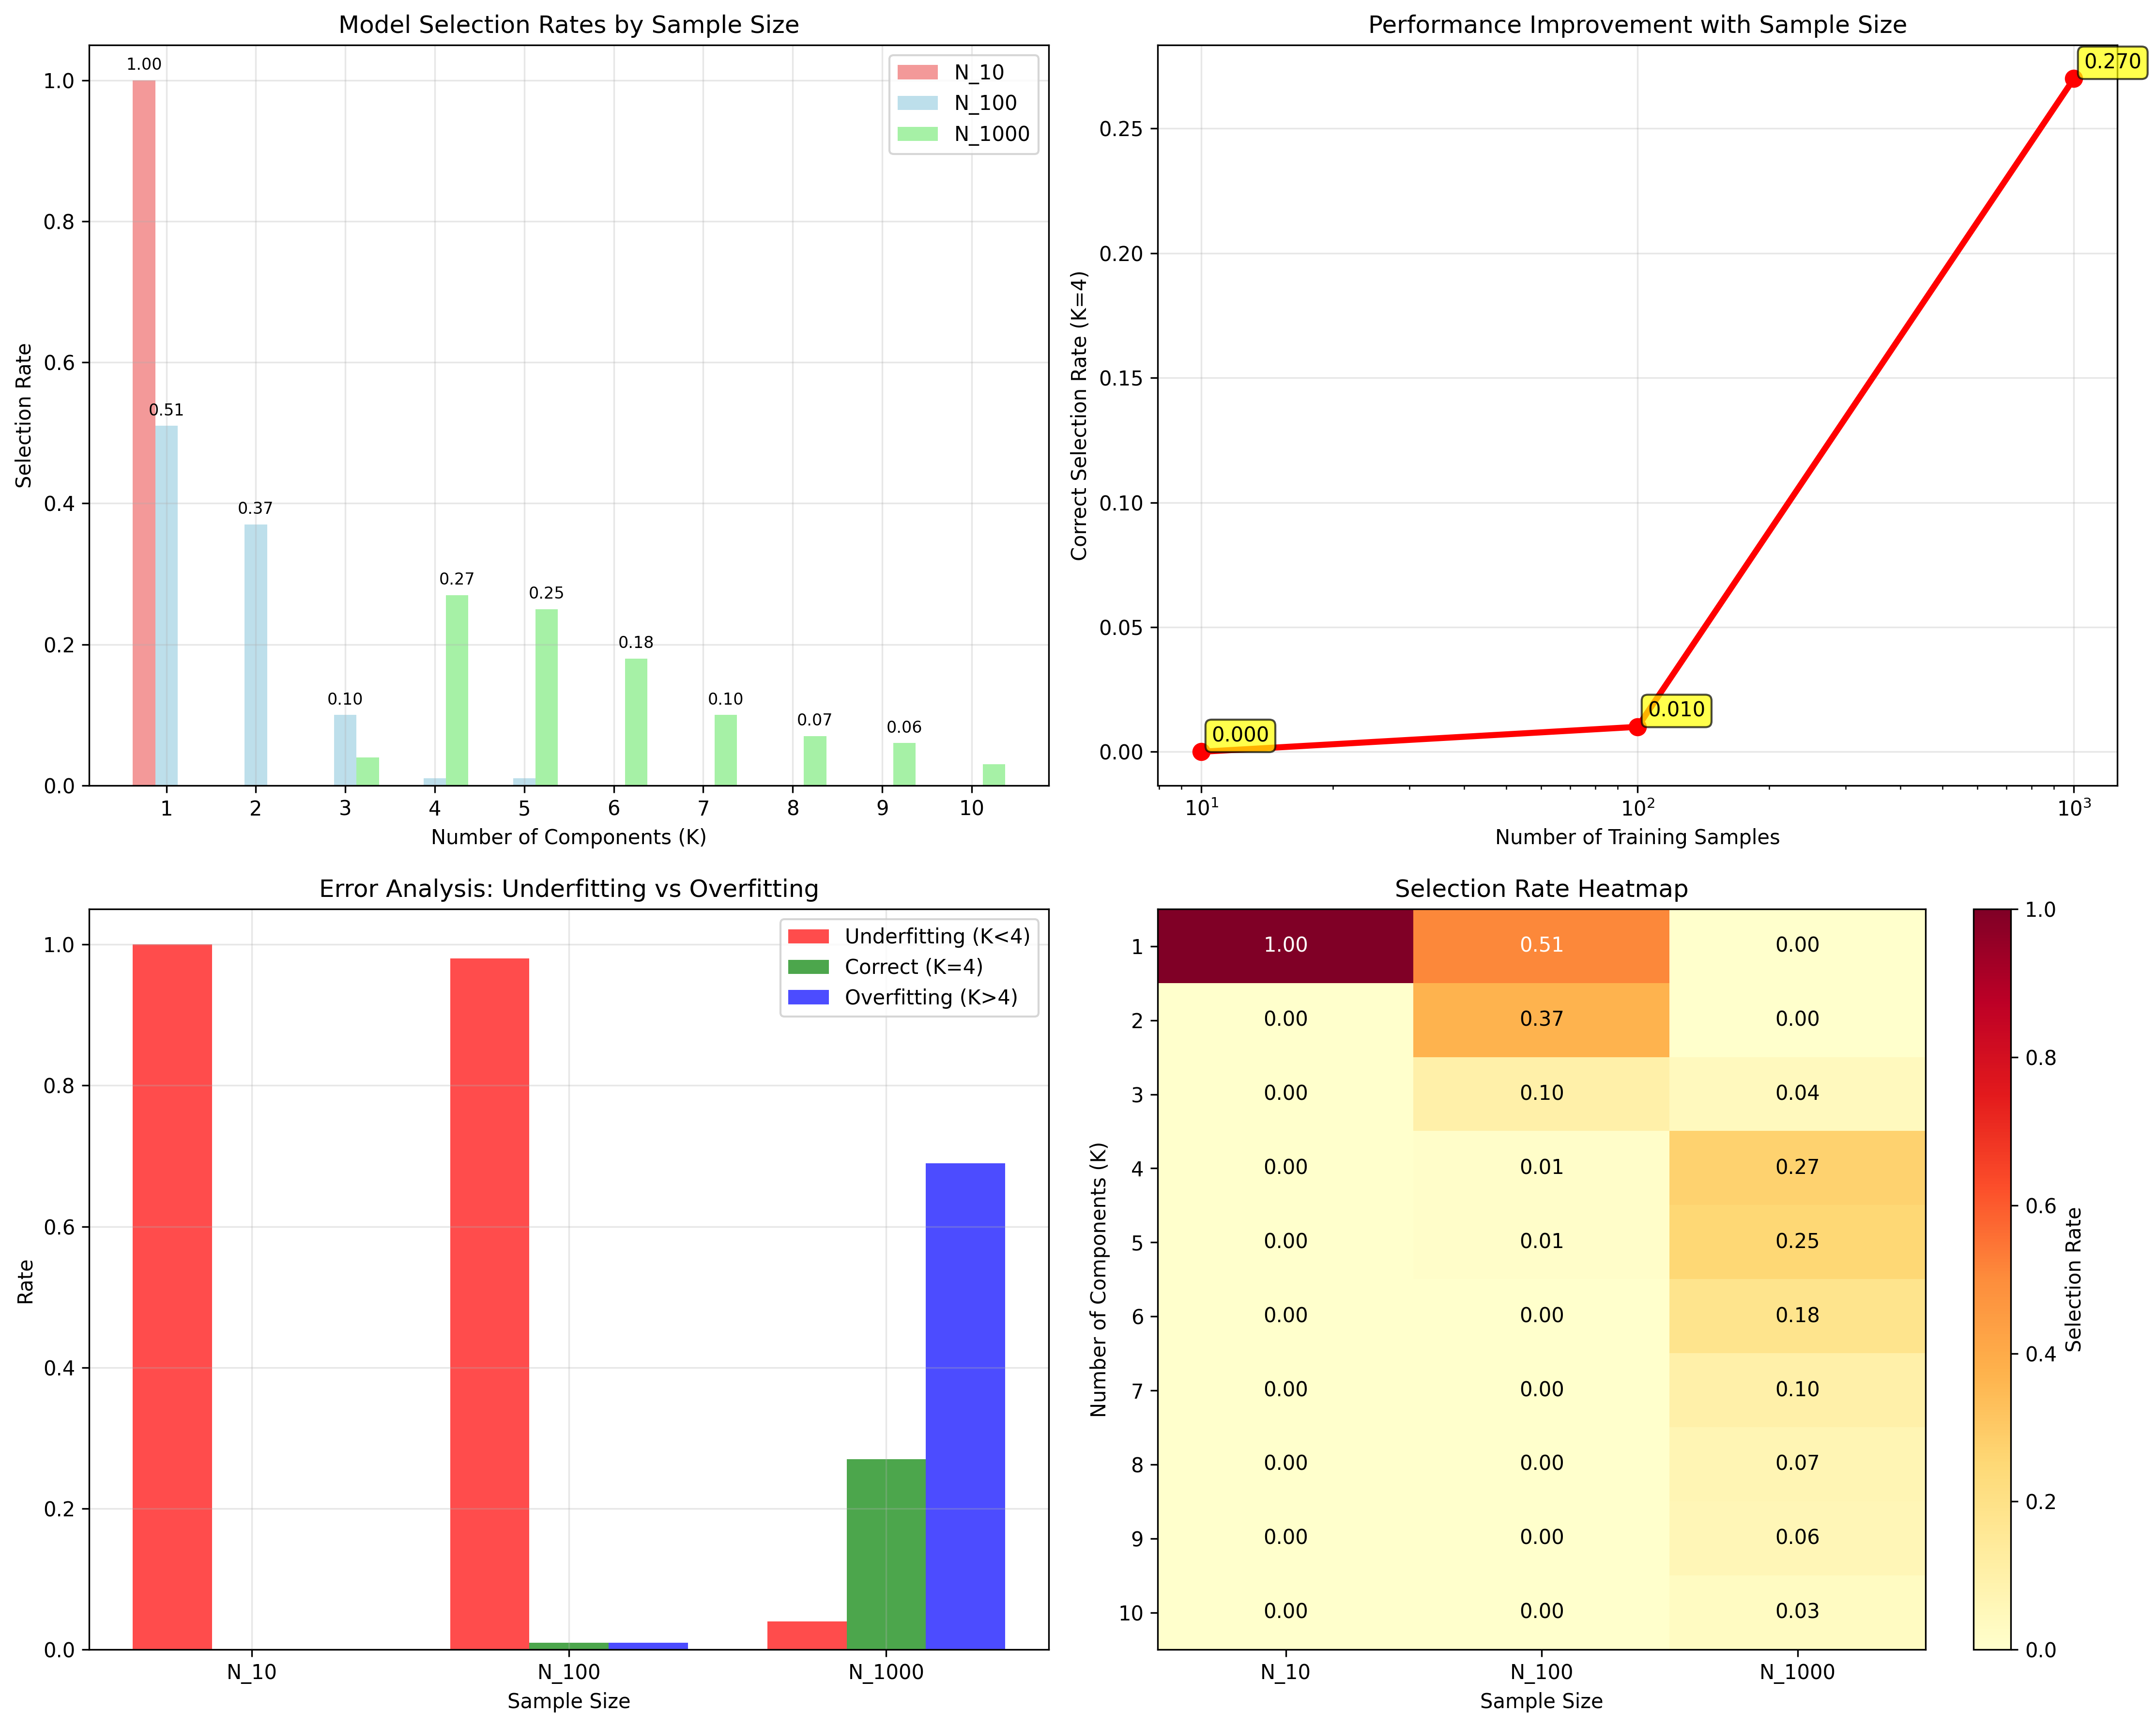
\includegraphics[width=0.8\textwidth]{gmm_selection_rates.png}
    \caption{Model selection performance: (a) Selection rates by sample size, (b) Correct selection rate vs sample size, (c) Underfitting/overfitting analysis, (d) Selection rate heatmap}
    \label{fig:selection_rates}
\end{figure}

\subsection{Discussion}

The experimental results reveal significant challenges in GMM model selection, with performance varying dramatically across sample sizes. With minimal data (N=10), the procedure completely fails to identify the true model, selecting only K=1 in all 100 repetitions. This extreme underfitting reflects the fundamental limitation of having only 10 data points to characterize a 4-component mixture in 2D space.

At N=100, performance improves slightly but remains poor, with 98\% underfitting and only 1\% correct selection. The model predominantly chooses oversimplified configurations (K=1: 51\%, K=2: 37\%), suggesting that while additional data provides some discrimination capability, it remains insufficient to reliably identify the true four-component structure.

Most notably, at N=1000 we observe a dramatic shift toward overfitting, with 69\% of selections choosing overly complex models (K>4) compared to only 27\% correct selections. This pattern indicates that with sufficient data, the cross-validation procedure becomes sensitive to capturing noise and minor variations rather than the true underlying structure. The true K=4 emerges as the most frequent choice (27\%), but faces strong competition from adjacent complexities (K=5: 25\%, K=6: 18\%).

From an implementation perspective, the loop-based Gaussian PDF calculations proved computationally intensive. Given more development time, I could have implemented a vectorized version using log-domain computations with the log-sum-exp trick for numerical stability. This would involve computing all component log-probabilities simultaneously via broadcasting and careful linear algebra operations, potentially achieving similar performance to optimized libraries while maintaining full control over the implementation.

The EM algorithm's sensitivity to initialization and local optima likely contributes to the variability in results, particularly for intermediate sample sizes. The observed pattern—transitioning from extreme underfitting through moderate performance to significant overfitting—highlights the delicate balance required in model selection and suggests that cross-validation alone may be insufficient for reliable GMM complexity determination without additional regularization or model selection criteria.

\subsection{Conclusion}
This study demonstrates the inherent challenges in GMM model selection, where cross-validation struggles to balance underfitting and overfitting across sample sizes. The results reveal that standard cross-validation alone is insufficient for reliable mixture complexity determination, particularly given the sensitivity to initialization and computational limitations. 

% =============================================================================
% APPENDIX
% =============================================================================
\newpage
\section*{Appendix: Code Repository}
\label{sec:appendix}

The complete Python implementation for this assignment is available at: \\
\url{https://github.com/GuestAGuy/EECE5644/tree/main/HW3}

The following files are the work for question 1 located in HW3Q1 folder
\begin{itemize}
    \item \texttt{Data\_Generation.py} - Generates 4-class Gaussian datasets and adjusts parameters
    \item \texttt{Theoretical\_Optimal\_Classifier.py} - Implements Bayesian optimal classifier
    \item \texttt{MLP.py} - Trains MLP models with cross-validation and evaluates performance
\end{itemize}

The following files are the work for question 2 located in HW3Q2 folder
\begin{itemize}
    \item \texttt{Data\_GenerationGMM.py} — true GMM definition, dataset generation, visualization, and saving of datasets.
    \item \texttt{Model\_Selection\_GMM.py} — EM implementation, training, 10-fold cross-validation, result aggregation, and plotting. 
\end{itemize}
% =============================================================================
% CITATIONS
% =============================================================================
\newpage
\section*{Citations and External Assistance}

\subsection*{External Resources}
\begin{itemize}
    \item Course lectures and notes for theoretical foundations
    \item Scikit-learn documentation for MLP implementation
    \item Scipy documentation for statistical functions
    \item Matplotlib documentation for visualization
    \item code written in earlier homeworks
\end{itemize}

\subsection*{AI Assistance}
This assignment was completed with assistance from AI tools for:
\begin{itemize}
    \item Conceptual clarification
    \item Debugging assistance with cross-validation implementation
    \item Visualization of plots
    \item LaTeX document structure
\end{itemize}

All mathematical derivations, experimental design, implementation, analysis, and final conclusions are my own work. AI assistance was used as a reference for clarification, debugging, and latex.

\end{document}